
Replay is an example of low-effort spoofing attacks; they require simply the replaying of a previously captured speech signal. Replay attacks can be realised with increasing ease, considering the widespread availability of mobile devices with reasonable quality in-built speakers (and microphones). The risk of playback attacks is even higher if recordings of a speaker are publicly available, and if text-independent system is used. Paradoxically, increased effectiveness of channel-compensation techniques and methods for compensating intersession variability can actually work in favour of the replay attack. All these factors show the increasing threat of replay attack on speaker verification systems and justify the importance of research on replay and replay countermeasures.

When modelling a replay attack one should take into account the impact of the following elements:
\begin{itemize}
\item acoustic effects introduced by the recording device;
\item acoustic conditions in the environment where the voice was acquired;
\item acoustic effects of the replay device, and the
\item acoustic conditions in the environment where the attack takes place. 
\end{itemize}

\begin{figure}
	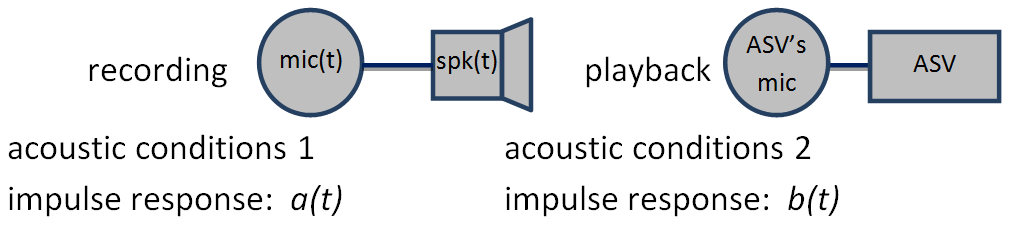
\includegraphics[width=1\linewidth]{Figs/replay.png}

	\caption{Schematic diagram of replay.}
	\label{fig::Replay}
\end{figure}


If $x(t)$ is the speech signal of the client, the playback (spoofing) signal $y(t)$ can be represented by:

\begin{equation}
y(t) = x(t)* mic(t) * a(t) * spk(t) * b(t)
\label{eq::playback}
\end{equation}

where * denotes convolution, $mic(t)$ and $spk(t)$ are impulse responses of the microphone and the speaker, respectively, and $a(t)$ and $b(t)$ are impulse responses of recording and replay environments, respectively (see Fig.~\ref{fig::Replay}). 

\subsection{Research on replay spoofing and replay countermeasures}

While a great deal of attention has been paid to medium- and high-effort spoofing algorithms (a thorough review of these can be found, e.g., in ~\cite{interspeechSpecialSession}), surprisingly, only few studies have been published so far on replay spoofing. The work in~\cite{Lindberg1999} assessed the vulnerabilities of an HMM-based text-dependent ASV system with concatenated digits. They showed that replay attacks are highly effective, but their experiments related to only two speakers. In the study of~\cite{Villalba2010} several playback cases were analysed: recording using a close-talk or a far-field microphone and transmission over an analogue or digital channel. Using their own corpus with five speakers the work showed that a joint factor analysis (JFA) ASV system is vulnerable to replay attacks -- the FAR at the EER threshold increased from 1\% to almost 70\%. 

Some measures were also proposed to prevent replay attacks. As far as text-dependent ASV systems are concerned, one of them is the use of challenge-response systems, which require the speaker to utter an ad hoc phrase which may not be easily expected. Another method which was developed for text-dependent systems (but may be easily adopted for text-independent systems) is based on comparing a new access trial with stored previous attempts ~\cite{Shang2010}. The experiments showed that this method caused a decrease in EER in  most of the cases, however, this method is useless if there were no previous access trials with a given recording. In other work~\cite{Wang2011} measuring of the channel noise is proposed in order to find a difference between the expected (simpler) channel and the more noisy replay channel, which includes also the recording device. The authors proposed two variants of their countermeasure, and they managed to decrease the EER from 40\% to 10\% with a baseline GMM-UBM system under replay spoofing.

Villalba and Lleida~\cite{Villalba2011} proposed a countermeasure which was based on detecting far-field recordings, bearing in mind that both telephone-based ASV systems and stand-alone ASV systems (e.g., installed at the entrance to a room) expect close-talk speech. The authors observed that far-field recordings cause changes in speech signal envelope; therefore they extracted 12 parameters describing the envelope and, based on them, trained a binary SVM classifier in order to discriminate far-field speech from close-talk speech. The authors claimed that they reached the far-field recognition rate of more than 90\%.


\subsection{Replay vs. other spoofing algorithms}
\label{sec::algorithms::playback}


\begin{table*}
%\ninept
\begin{center}
    \begin{tabular}{ l | c c c c }
    \hline
     	 Attack & Na\"{i}ve impostor &  Replay & Voice conversion & Speech synthesis\\ 
    \hline
  Speech used & \begin{tabular}{ c } impostor's\\(genuine) \end{tabular} & client's &  \begin{tabular}{ c } impostor's\\(converted) \end{tabular} & synthetic\\
Effort & zero & low & medium-high & high\\
Effectiveness & low &  \textbf{(?)} & medium-high & high\\
 \hline
\hline
    \end{tabular}
    \caption{Comparison of four different attacks in terms of speech used,  required effort and effectiveness.}
		\label{tab::attacks}
   \end{center}
\end{table*}


Table \ref{tab::attacks} shows a comparison of replay spoofing and na\"{i}ve (zero-effort) impostors, voice conversion and speech synthesis. The attacks are ordered in terms of the effort involved in each case. Replay attacks require slightly increased effort compared to na\"{i}ve imposture (need for target voice acquisition and replay hardware). Voice conversion and speech synthesis require specialised algorithms, in addition to appropriate hardware and parameters describing the target voice. They belong to a class of higher-effort spoofing attacks. While voice conversion is still based upon the conversion of an original speech signal, speech synthesis starts with text input. In this sense the attack requires the most effort of all to implement successfully. One may reasonably suppose that the effectiveness of each attack is linked to the effort involved; the higher the effort, the greater the impact on ASV performance. This hypothesis will be verified later in this work.

\subsection{Voice conversion}
\label{ssec:vconv}

We used the approach to voice conversion originally presented in~\cite{Matrouf2005}. At the frame level, the speech signal of a spoofer denoted by $y(t)$ is filtered in the spectral domain as follows:

\begin{equation}
Y'(f) = \frac{\left|H_{x}(f)\right|}{\left|H_{y}(f)\right|}Y(f)
\label{eq:conversioneq}
\end{equation}

\noindent where $H_{x}(f)$ and $H_{y}(f)$ are the vocal tract transfer functions of the targeted speaker and the spoofer respectively.  $Y(f)$ is the spoofer's speech signal whereas $Y'(f)$ denotes the result after voice conversion.  As such, $y(t)$ is mapped or converted towards the target in a spectral-envelope sense, which is sufficient to overcome most ASV systems. 

$H_x(f)$ is determined from a set of two Gaussian mixture models (GMMs).  The first, denoted as the automatic speaker recognition (asr) model in the original work, is related to ASV feature space and utilised for the calculation of a posteriori probabilities whereas the second, denoted as the filtering (fil) model, is a tied model of linear predictive cepstral coding (LPCC) coefficients from which $H_x(f)$ is derived.  LPCC filter parameters are obtained according to:

\begin{equation}
x_{fil} = \sum\limits_{i=1}^{M}p(g_{asr}^{i}|y_{asr}) \mu_{fil}^{i}
\label{eq:EMit}
\end{equation}

\noindent where $p(g_{asr}^{i}|y_{asr})$ is the a posteriori probability of Gaussian component $g_{asr}^{i}$ given the frame $y_{asr}$ and $\mu_{fil}^{i}$ is the mean of component $g_{fil}^{i}$ which is tied to $g_{asr}^{i}$.  $H_{x}(f)$ is estimated from $x_{fil}$ using an LPCC-to-LPC transformation and a time-domain signal is synthesised from converted frames with a standard overlap-add technique. Full details can be found in~\cite{Matrouf2005,Bonastre2006,Bonastre2007}.


\subsection{Speech synthesis}

There is a large variety of speech synthesis algorithms, such as formant, diphone or unit-selection based synthesis. State-of-the-art text-to-speech systems use either unit-selection or the hidden Markov model-based synthesis (HTS). Whilst the former requires large amounts of speech data, the latter does not, and can therefore much more easily generate speech targeted towards a specific client. 

Accordingly, in this paper we consider spoofing with HTS synthesis, following the approach described in~\cite{Yamagishi2009}, and using the HMM-based Speech Synthesis System (HTS)\footnote{http://hts.sp.nitech.ac.jp/}. Parametrisation includes STRAIGHT (Speech Transformation and Representation using Adaptive Interpolation of weiGHTed spectrum) features, Mel-cepstrum coefficients and the logarithm of the fundamental frequency (log $F_{0}$) with their delta and acceleration coefficients. Acoustic spectral characteristics and duration probabilities are modelled using multispace distribution hidden semi-Markov models (MSD-HSMM)~\cite{Russell1985}.  Speaker dependent  excitation, spectral and duration models are adapted from corresponding independent models according to a speaker adaptation strategy referred to as constrained structural maximum a posteriori linear regression (CSMAPLR)~\cite{Yamagishi2009a}.  Finally, time domain signals are synthesised using a vocoder based on Mel-logarithmic spectrum approximation (MLSA) filters.  They correspond to STRAIGHT Mel-cepstral coefficients and are driven by a mixed excitation signal and waveforms reconstructed using the pitch synchronous overlap add (PSOLA) method.


\subsection{Aim of this work}

This paper aims at analysing threat of replay attacks when using large speaker databases and most effective speaker verification systems, and compare it with the threat of other spoofing algorithms: voice conversion and speech synthesis. The impact of acoustic environment and playback devices on performance of speaker verification systems will be investigated. 

This work will also verify the effectiveness of replay detection, using the previously described replay countermeasure ~\cite{Villalba2011}, which had been  shown to be effective in detecting far-field recordings. Therefore, we are going to identify a relative threat of replay using the state-of-the-art ASV systems and a replay countermeasure.

